\chapter{Radar Background}
\label{radar_background}
Radars come in a variety of forms, but for this work we are primarily concerned with pulsed monostatic radars. In this mode of operation, a radar transmits a pulse of electromagnetic energy and then switches to a listening mode to record the signal from any resulting reflections. The received power $P_r$ backscattered from a target is described by the radar equation \autocite{Sko01}:
\begin{equation}\label{eq:radar_equation}
 P_r = \frac{P_t G}{4\pi r^2} \times \sigma \times \frac{A_e}{4\pi r^2}.
\end{equation}
The transmitted power $P_t$ is concentrated by the antenna with a gain of $G$, but it also decays with distance (or range) $r$ according to $1/(4\pi r^2)$ as it spreads into space. The target then scatters a fraction of the power, the target's radar cross section $\sigma$, back toward the radar. The backscattered power once again decreases with range $r$ before returning to the antenna and experiencing a gain dependent on the effective aperture area $A_e$. In this monostatic case with the transmitting and receiving antenna co-located, the aperture is related to the transmitting gain by $G = 4\pi A_e/\lambda^2$, where $\lambda$ is the wavelength of the radio wave. Though it is important to remember how the received power relates to the radar's power and gain parameters ($P_t$, $G$, $A_e$) and the target's cross section and range ($\sigma$, $r$), we will mostly be able to ignore these effects by working only in terms of the received power as a function of range or, equivalently, time delay.

Once a pulse is sent and the received signal is recorded for as long as desired, the process is repeated to monitor how the radar targets change over time. The time from one pulse to the next is called the \emph{pulse period} and its inverse the \emph{pulse repetition frequency} (PRF). The PRF is an important parameter in the design of a radar experiment since it specifies the amount of time during which the radar can listen for reflections. Hence, it also gives the maximum unambiguous distance at which targets can be measured. For ionospheric experiments, pulse periods on the order of one to ten milliseconds, at a minimum, are common. With a zenith-pointing radar, one millisecond corresponds to a maximum unambiguous range of 150 km, which falls in the E-region (the total distance traveled by a returning wave in 1 ms is $c [m/s] * 1e^{-3} [s] \approx 300 [km]$ where $c \approx 3e8 [m/s]$ is the speed of light, so the maximum range is half that).

Usually these pulsed monostatic radars operate at a fixed frequency, or multiple fixed frequencies in independent channels. Data is typically acquired by sampling the received waveform so that its zero frequency corresponds to the radar's baseband frequency. This frequency shift is accomplished either directly in the digital domain after high-frequency sampling or with analog filtering and mixing \autocite{Ric05, Sko08}. Either way, the end result is a digitally sampled signal of complex numbers encoding the magnitude and phase of the received signal, a vector that can be stored and further analyzed to extract information about the radar scene. We employ the following notation for representing the transmitted and received radar signals: the transmitted waveform is represented by the complex sequence $s[l]$ with $L$ elements and indices $l=0,\dotsc,L-1$; the received waveform is represented by the complex sequence $y[m]$ with $M$ elements and indices $m=0,\dotsc,M-1$. For consistency, we will always use $l$ to index the transmitter sequence, $m$ to index the received sequence, and the corresponding capital letters to denote the respective sequence lengths.

\section{Pulse Design}
\label{pulse_design}
While design parameters like the pulse period and system parameters like the transmitter power and antenna gain are important in designing a radar experiment, the pulse itself is critical. Imagine the pulse as a square wave centered at the radar's operating frequency as shown in Figure \ref{fig:pulse_returns}. In this figure, the delay space is divided into samples according to the sampling period, and the transmitted and received waveforms are shown along with their vector counterparts. The waveforms display a fixed frequency, the radar operating frequency, but are modulated on and off according to the pulse length. Although the ideal on/off of a square wave is never achieved in practice, it is a convenient way to conceptualize the waveforms.
\begin{figure}[tpb]
 \centering
 \begin{subfigure}{0.5\textwidth}
  \centering
  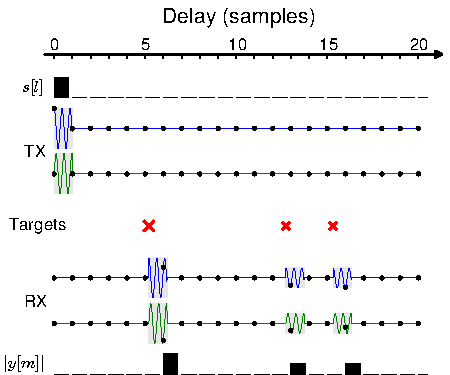
\includegraphics{shortpulse_return}
  \caption{Short pulse}
  \label{fig:short_pulse_return}
 \end{subfigure}%
 \begin{subfigure}{0.5\textwidth}
  \centering
  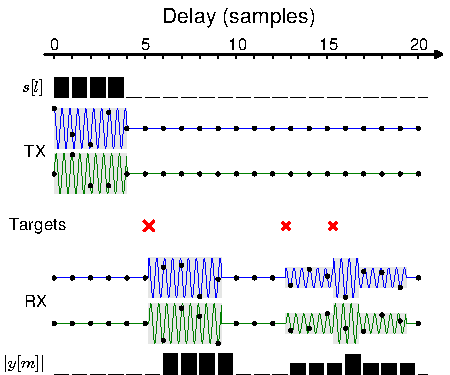
\includegraphics{longpulse_return}
  \caption{Long pulse}
  \label{fig:long_pulse_return}
 \end{subfigure}
 \caption[Transmitted and received signals for a short and long pulse]{\emph{Transmitted and received signals for a short and long pulse.} In each case, transmitted (TX) and received (RX) waveforms are shown as a function of delay along with the corresponding sampled baseband signals $s[l]$ and $y[m]$. Each waveform has an in-phase (blue) and quadrature (green) component, representing the wave's magnitude and phase when thought of as the real and imaginary parts of the complex signal. The received waveform encapsulates the delays and magnitude differences applied to the transmitted pulse by three point targets. Because of ambiguity created by the pulse length, the received signal for the short pulse is easier to interpret than for the long pulse, but the long pulse allows for increased total power through averaging over multiple samples.}
 \label{fig:pulse_returns}
\end{figure}%

\subsection{Pulse Length}
The simplest mode of operation matches the length of the transmitted pulse with the sampling rate of the received signal. In this way, each sample represents the sum of reflections over a particular range window with width corresponding to the pulse length. This short pulse mode of operation is depicted in Figure \ref{fig:short_pulse_return}, where three point targets appear individually as three nonzero samples in the received signal. In general, range resolution is defined by the sampling rate, while range ambiguity, or the interference region for multiple scatterers, is defined by the pulse length. In the short pulse case, the range resolution matches the range ambiguity so that the ambiguity does not pose an interpretation problem.

The primary downside of a short pulse is that it limits the sensitivity of the radar in terms of energy on target. Since the peak power of a pulse is limited by the physical radar equipment, the only way to increase the total power is to increase the pulse length. With a pulse greater than the sampling period, one can add the returned signal over multiple samples within the pulse to achieve a higher sensitivity due to higher total power. However, a longer pulse also increases the range ambiguity of the measurement since the return from any single target will affect multiple receiver samples. This long-pulse mode of operation is depicted in Figure \ref{fig:long_pulse_return}. The example shows both the positives and negatives of a longer pulse: more samples for increased sensitivity with the first target, but ambiguity in the received signal between the latter two closely-spaced targets.

Two additional points are relevant when discussing pulse length: transmitter duty cycle and Fourier frequency resolution. In order to transmit large amounts of power instantaneously, transmitters often have a maximum duty cycle that describes the fraction of time that the transmitter is allowed to be on. A duty cycle is necessary so that there is enough off time to build up the power supply and allow physical components to cool. Because of these requirements, the pulse length cannot be increased indiscriminately and has a fixed limit with respect to the pulse period. The other consideration is Fourier frequency resolution. For persistent targets, pulse-to-pulse Fourier analysis is possible to measure how the target evolves in time, with the maximum observable frequency component given by half the pulse repetition frequency. For quickly-evolving or transient targets, the pulse-to-pulse method of Fourier analysis is not sufficient and intra-pulse Fourier analysis is necessary. In that case, the maximum observable frequency is half the sampling frequency and the resolution is the inverse of the pulse length. Thus, increasing the pulse length also has the benefit of improving the frequency resolution of intra-pulse Fourier analysis.

\subsection{Pulse Waveforms}
One way to deal with the ambiguity problem is to code the pulse by modulating it with a designed waveform. Because of the way that coding allows for concentration of the pulse energy after decoding, this process is often called \emph{pulse compression}. One simple and widespread method is linear frequency modulation (LFM), also known as a chirp waveform. A chirp pulse starts off at a low frequency and linearly increases in frequency over time to a high frequency, or vice-versa. An example is given in Figure \ref{fig:lfm_chirp}.
\begin{figure}[tpb]
 \centering
 \begin{subfigure}{\textwidth}
  \centering
  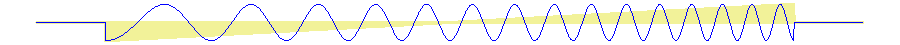
\includegraphics{lfmpulse}
  \caption{LFM Chirp}
  \label{fig:lfm_chirp}
 \end{subfigure}
 
 \vspace{\baselineskip}
 \begin{subfigure}{\textwidth}
  \centering
  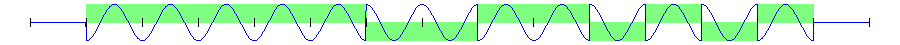
\includegraphics{barker13pulse}
  \caption{Barker-13}
  \label{fig:barker13_pulse}
 \end{subfigure}
 
 \vspace{\baselineskip}
 \begin{subfigure}{\textwidth}
  \centering
  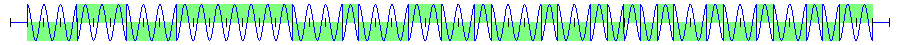
\includegraphics{mslpulse}
  \caption{Minimum peak sidelobe (51 bauds)}
  \label{fig:msl_pulse}
 \end{subfigure}
 \caption[Waveform encoding examples]{\emph{Waveform encoding examples.} These pulse waveforms depict three commonly used encodings: \textbf{(\subref{fig:lfm_chirp})} an LFM chirp pulse with a linear frequency sweep from low to high, \textbf{(\subref{fig:barker13_pulse})} a binary phase-coded pulse using the Barker-13 code, and \textbf{(\subref{fig:msl_pulse})} a binary phase-coded pulse using a minimum peak sidelobe code with 51 bauds. The yellow fill in the background of \textbf{(\subref{fig:lfm_chirp})} indicates the pulse's frequency with respect to the baseband, while the green rectangles in \textbf{(\subref{fig:barker13_pulse})} and \textbf{(\subref{fig:msl_pulse})} indicate the positive or negative phase of each baud.}
 \label{fig:waveform_encodings}
\end{figure}%
Another common form of modulation is to divide the pulse into equal length segments called \emph{bauds} and encode using the phase of each baud. Often the codes use only two opposite phases (e.g. $1$ and $-1$) and the process is called binary phase coding, but the use of more phases is certainly possible. Two examples of commonly-used and well-behaved binary phase codes are shown in Figure \ref{fig:waveform_encodings}. The Barker-13 code of Figure \ref{fig:barker13_pulse} has 13 bauds with phases described by the binary sequence
\begin{equation}
 s_{\text{B}_\text{13}} = 1111100110101,
\end{equation}
while the minimum peak sidelobe code of Figure \ref{fig:msl_pulse} has 51 bauds with phases described by the binary sequence
\begin{equation}
 s_{\text{MSL}_\text{51}} = 000111000111111100010001100100010010101001001001011.
\end{equation}

\section{Matched Filtering}
\label{matched_filtering}
When coded pulses are used, or even just long pulses, one needs a way to decode the received result and integrate the distributed power. The intuitive way of doing this, by starting with each sample in the received signal and operating over a window the length of the pulse to reverse the effects of the code and sum the result, is called a \emph{matched filter}. Stated another way, the matched filter correlates every segment of the received signal with the transmitted pulse. Mathematically, the matched filter performs the correlation
\begin{align}
 u[p] &= \sum_{m=0}^{M-1} s^*[m - p + (L-1)] y[m]
 \intertext{or equivalently}
 u[p] &= \sum_{l=0}^{L-1} s^*[l] y[p + l - (L-1)],
\end{align}
where $s^*$ signifies the complex conjugate of the code $s$ and the matched filter result is denoted by $u[p]$ for $p=0,\ldots,P-1$ with $P=M+L-1$. These equations reference "out of bounds" indices of $y[m]$ and $s^*[l]$; for simplicity we take the convention that any out of bounds values are zero. The correlation process of the matched filter is shown in Figure \ref{fig:barker13_autocorrelation} in the context of autocorrelation of the Barker-13 code, which corresponds to the ideal case when the received signal is due to perfect reflection from a point target.
\begin{figure}[ptb]
 \centering
 \begin{tabular}{cc}
  $p=0$ & \raisebox{-0.5\height}{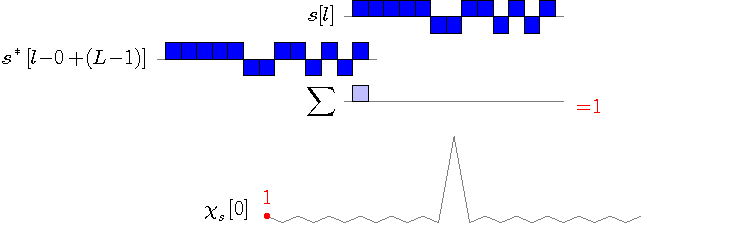
\includegraphics{autocorrelation_b13_0}}\\[\dimexpr-\baselineskip]
  \hline\\
  $p=1$ & \raisebox{-0.5\height}{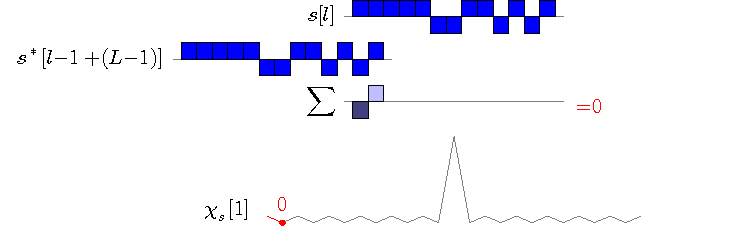
\includegraphics{autocorrelation_b13_1}}\\
  \hline\\
  $p=6$ & \raisebox{-0.5\height}{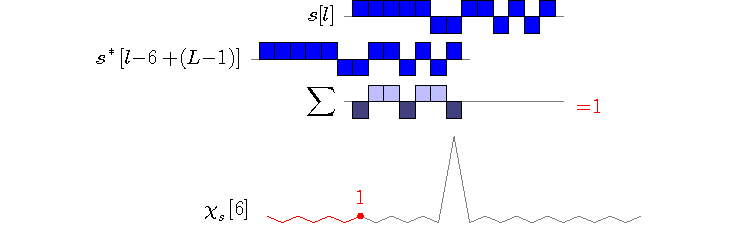
\includegraphics{autocorrelation_b13_6}}\\
  \hline\\
  $p=12$ & \raisebox{-0.5\height}{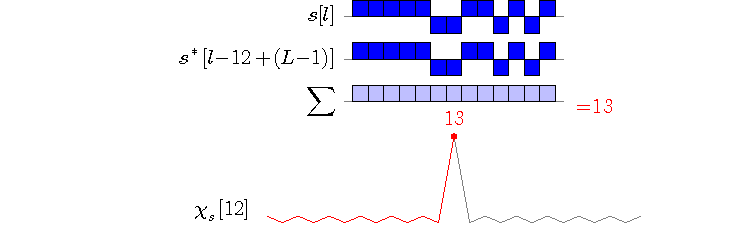
\includegraphics{autocorrelation_b13_12}}
 \end{tabular}
 \caption[Autocorrelation of the Barker-13 code]{\emph{Autocorrelation of the Barker-13 code.} Each panel depicts the calculation of a single sample $p$ for the autocorrelation of the Barker-13 code. The first two lines of each panel show the code sequence $s[l]$ and its shifted conjugate. The third line shows the resulting multiplication of the first two lines and sum total of the values. The fourth line gives a plot of the autocorrelation, highlighting the calculated sample.}
 \label{fig:barker13_autocorrelation}
\end{figure}%
The benefits of the matched filter are its sensitivity and ease of computation: it produces the optimal signal-to-noise ratio (SNR) when decoding point targets and takes the form of a simple linear filter.

There is one degree of freedom when computing the matched filter: one can scale the code $s$ by any amount and still have optimal SNR at the output. This is because increasing $s$ by a scalar quantity not only increases the magnitude of the output when run against a matching sequence, but it also equally increases the magnitude of the output when run against non-matching random noise. Since the output is typically examined in terms of SNR, this arbitrary scaling makes no difference to the analysis. In a practical sense, however, it is often convenient to scale the code $s$ so that it has an $l_2$ norm of one:
\begin{equation}\label{eq:scaled_code}
 s'[l] = \frac{s[l]}{\sqrt{\sum_{k=0}^{L-1} \abs{s[k]}^2}}.
\end{equation}
When this is done, noise at the output of the matched filter has the same average power as noise at the input, and no recalculation of the noise power is necessary to compute SNR.

\subsection{Autocorrelation and Range Sidelobes}
Since targets essentially reflect the transmitted signal, just with phase and power differences and mixing from multiple or distributed targets, we can examine the effect of matched filtering by looking at a code's autocorrelation:
\begin{equation}
 \chi_s[p] = \sum_{l=0}^{L-1} s[l] s^*[l - p + (L-1)],
\end{equation}
where $p=0,\ldots,P-1$ with $P=2L-1$. As shown in Figure \ref{fig:barker13_autocorrelation} for the Barker-13 code, the autocorrelation of any code has a peak in the middle, corresponding to when the received and transmitted codes are perfectly aligned. In the matched filter result, the peak occurs at the delay, or range, corresponding to the location of the reflecting target. Away from the peak, the autocorrelation is not zero but rather some pattern of varying response that depends on the code. When these off-peak responses are seen in the matched filter result, they are called \emph{range sidelobes}.

Particular codes are selected for use because of their autocorrelation properties, where keeping sidelobe response to a minimum is desirable to minimize ambiguity and artifacts. The Barker-13 code is the longest in a class of Barker codes of differing lengths that have a maximum sidelobe level of one. It is possible to enforce similar minimum peak sidelobe performance for codes of other (particularly longer) lengths; these are unsurprisingly called minimum peak sidelobe codes, and they have been found through simple brute force search \autocite{Lin75,CFB90,CHC01,CR05}. The 51-baud example given in Figure \ref{fig:msl_pulse} is just one of the codes of different lengths with the minimum peak sidelobe property. The LFM chirp that we encountered earlier also has well-behaved range sidelobes, and in that case they decay from the peak according to a sinc function.

\subsection{Frequency Banks of Matched Filters}
Moving targets complicate the use of a matched filter to decode the received signal because the Doppler frequency shift causes a mismatch. If a target is moving toward (away from) the radar, the reflected signal is shifted up (down) in frequency. In order to correlate properly, the matched filter needs to be similarly frequency shifted. Of course, the true frequency shift due to target motion is not known ahead of time, so it is another unknown that must be determined along with the target's range. We cope with this problem by processing the received signal with a bank of filters, each with a different frequency shift. Computationally, it is convenient to have these filters be equally spaced in frequency up to the maximum detectable frequency shift, determined from the sample rate according to the Nyquist criterion. When that is done, the filter bank can be computed efficiently through the Discrete Fourier Transform (DFT). The equation describing the matched filter bank is similar to the single matched filter:
\begin{align}
 u[n,p] &= \sum_{m=0}^{M-1} s^*[m - p + L-1]\, e^{-2\pi i n (m-p+L-1)/N}\, y[m]\\
 \intertext{or equivalently}
 u[n,p] &= \sum_{l=0}^{L-1} s^*[l]\, e^{-2\pi i n l / N}\, y[p + l - (L-1)].
\end{align}
The difference, of course, is that for each of the $N$ frequencies indexed by $n$ for $0,\dotsc,N-1$, the transmitted code is modulated at that frequency before correlation with the received signal.

Visualizing the results of a filter bank also poses a challenge. Since we will frequently have to deal with this type of visualization, a brief discussion is in order. Often we want to plot data from multiple pulses in order to see how the targets vary over time. With a filter bank, that means plotting signal strength as a function of three variables: range, frequency, and time. A natural representation is a video, with each frame being a plot of signal strength as a function of range versus frequency for a single pulse. Of course, that has the distinct disadvantage of not working well in print. A more suitable approach is to truncate one of the dimensions in some way. If all of the targets have a negligible or similar Doppler shift, then it is reasonable to just plot the data for that one frequency. This results in a standard range-time-intensity (RTI) plot with range as the vertical axis, pulse time as the horizontal axis, and signal intensity represented by color or shading. Figure \ref{fig:electrojet_example} in the introduction is an example of this approach. However, when moving and stationary targets mix (as with the meteor head echo and trail shown in Figure \ref{fig:meteor_scattering_example}), single frequency truncation is insufficient. In those cases and when an RTI-type plot is desired, the single frequency that gives the maximum response over all ranges is selected for each pulse individually. Most of the time this is sufficient to produce a well-decoded plot, but it still fails when multiple frequency-shifted targets appear in the same pulse. There are other approaches for visualizing filter bank outputs, but here we will only employ the peak-frequency-response approach for RTI plots.

\section{Measurement Ambiguity}
\label{radar_ambiguity}
When analyzing the received radar signal for a single pulse, we are interested in how the transmitted signal was reflected as a function of delay (range) and frequency (range-rate). A frequency bank of matched filters produces a peak response at the delay and frequency of any target, but it also produces off-peak sidelobes as an artifact of the filtering process. The delay-frequency sidelobes can, depending on their magnitude, obscure weaker targets or bias the measurement through interference. We call these effects measurement ambiguity.

\subsection{Ambiguity Function}
As we saw in the single matched filter case, sidelobes are a consequence of the autocorrelation of a particular code. The same is true in the filter bank case, except we must consider the autocorrelation not only as a function of delay but as a function of frequency:
\begin{multline}
 \chi_s[n,p;n',p'] = \sum_{m=0}^{M-1} s[m - p' + L - 1]\, e^{2\pi i n' (m-p'+L-1)/N}\\
 \times s^*[m - p + L - 1]\, e^{-2\pi i n (m-p+L-1)/N}.
\end{multline}
It is necessary to explicitly write this function in terms of the two frequency indices $n$ and $n'$ and the two delay indices $p$ and $p'$ because of the nonlinear interaction between frequency and delay in the exponential term. As with before, $n,n' \in [0, N-1]$, $p,p' \in [0, P-1]$, and $M = P - (L-1)$. The delay-frequency autocorrelation of a code is also known as its \emph{ambiguity function}, although this term is sometimes used to denote the squared magnitude of the autocorrelation \autocite{Woo80}. The sidelobes of a code are completely described by the code's ambiguity function.

To make this concept more accessible, consider again the example codes encountered earlier. The ambiguity functions of the Barker-13, minimum sidelobe, and LFM chirp waveforms are shown in Figure \ref{fig:ambiguity_functions}.
\begin{figure}[tpb]
 \centering
 \begin{subfigure}{0.5\textwidth}
  \centering
  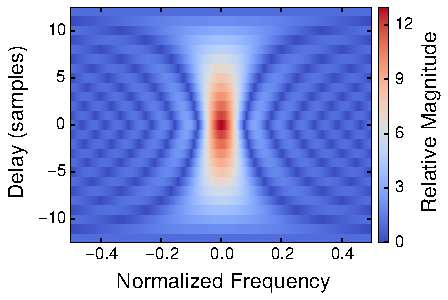
\includegraphics{ambiguity_uncoded}
  \caption{Uncoded pulse (13 samples long)}
  \label{fig:uncoded_ambiguity}
 \end{subfigure}%
 \begin{subfigure}{0.5\textwidth}
  \centering
  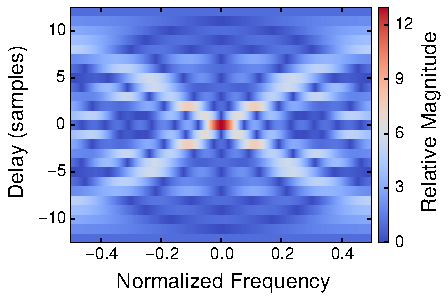
\includegraphics{ambiguity_barker13}
  \caption{Barker-13}
  \label{fig:barker13_ambiguity}
 \end{subfigure}
 
 \vspace{\baselineskip}
 \begin{subfigure}{0.5\textwidth}
  \centering
  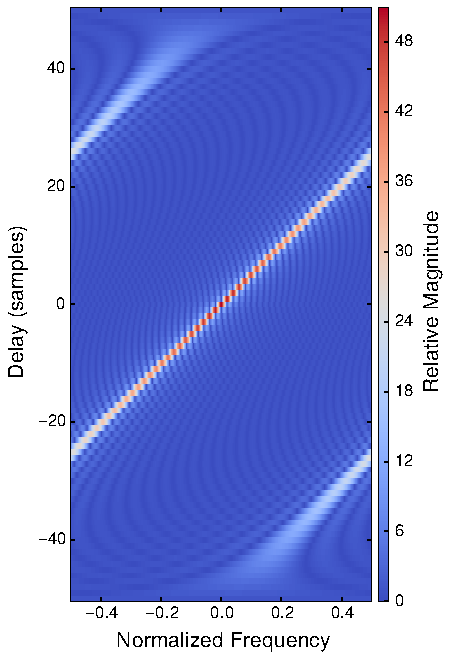
\includegraphics{ambiguity_lfm}
  \caption{LFM chirp (51 samples long)}
  \label{fig:lfm_ambiguity}
 \end{subfigure}%
 \begin{subfigure}{0.5\textwidth}
  \centering
  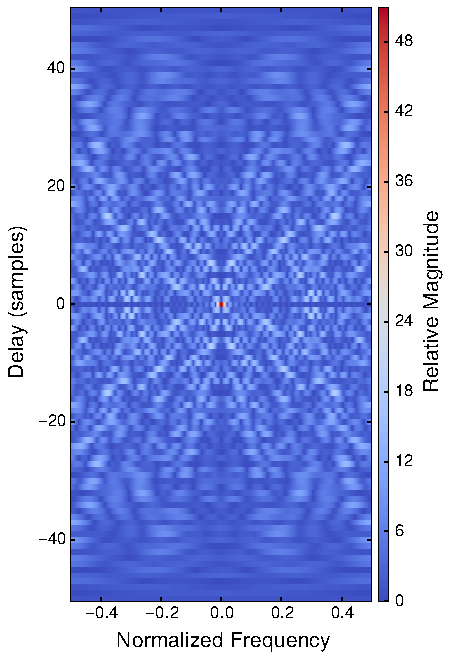
\includegraphics{ambiguity_msl}
  \caption{Minimum sidelobe (51 bauds)}
  \label{fig:msl_ambiguity}
 \end{subfigure}
 \caption[Ambiguity function examples]{\emph{Ambiguity function examples.} These delay-frequency images show the ambiguity function magnitude with $N=512$ frequencies for the \textbf{(\subref{fig:uncoded_ambiguity})} 13-sample uncoded pulse, \textbf{(\subref{fig:barker13_ambiguity})} Barker-13 code, \textbf{(\subref{fig:lfm_ambiguity})} 51-sample discretized LFM chirp with bandwidth equal to the sampling frequency, and \textbf{(\subref{fig:msl_ambiguity})} 51-baud minimum peak sidelobe code.}
 \label{fig:ambiguity_functions}
\end{figure}%
As a point of comparison, this figure also includes the ambiguity function of an uncoded pulse. All of the ambiguity functions have a peak centered at at zero delay and zero frequency, or rather the reflecting target's delay and frequency. The uncoded pulse has a strong response for many samples surrounding the peak: along the zero-frequency axis, the response decays linearly on both sides of the peak, while along the zero-delay axis, the response decays with the periodic sinc function. In contrast, the peaks for the Barker-13 and minimum sidelobe codes are well-defined and isolated with the sidelobe response lower but spread out across the delay-frequency space. The LFM chirp is interesting because of its ridge-like response, with strong ambiguity along a line in delay-frequency space but minimal sidelobes elsewhere. Thus, the LFM chirp is popular for use with a single matched filter since it is insensitive to frequency shifts (aside from a corresponding shift in the apparent target range).

\subsection{Sidelobes in Action}
The differences in ambiguity between these codes have a large impact in practice. Figures \ref{fig:meteor_uncoded_barker13} and \ref{fig:meteor_msl_lfm} show a meteor head echo and trail measured separately using the 50 MHz Jicamarca radar with a 40$\mu$s uncoded pulse, a 13$\mu$s Barker-13 pulse, a 51$\mu$s minimum sidelobe pulse with 51 bauds, and a 51$\mu$s LFM chirp with 1 MHz frequency sweep.
\begin{figure}[tpb]
 \begin{subfigure}{\textwidth}
  \centering
  \textsf{\footnotesize Mar 01 2011, 10:04:xx (s)}
  
  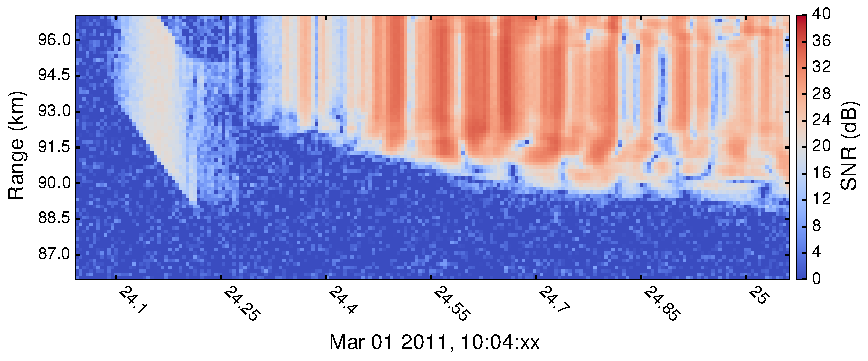
\includegraphics[trim=0px 20px 0px 3px,clip]{head_and_flare_rti_2}
  \caption{Uncoded pulse (40$\mu$s), unfiltered}
  \label{fig:meteor_uncoded_unfiltered}
 \end{subfigure}
 
 \vspace{0.5\baselineskip}
 \begin{subfigure}{\textwidth}
  \centering
  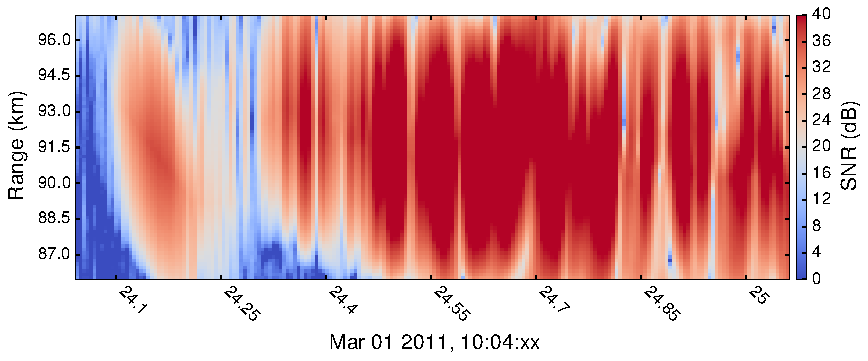
\includegraphics[trim=0px 20px 0px 3px,clip]{head_and_flare_mf_rti_2}
  \caption{Uncoded pulse (40$\mu$s), matched filter}
  \label{fig:meteor_uncoded_mf}
 \end{subfigure}
 \caption[Meteor head and trail measured with an uncoded pulse]{\emph{Meteor head and trail measured with an uncoded pulse.} These figures show the signal-to-noise ratio (SNR) as a function of range and time for one second of 1$\mu$s-sampled data taken with the 50 MHz Jicamarca radar. An uncoded pulse was used, with \textbf{(\subref{fig:meteor_uncoded_unfiltered})} showing the unfiltered result and \textbf{(\subref{fig:meteor_uncoded_mf})} showing the peak-frequency-response matched filter result. The SNR is low before filtering, but the range sidelobes resulting from the filter completely obscure the meteor trail.}
 \label{fig:meteor_uncoded_barker13}
\end{figure}%
\begin{figure}[tpb]
 \vspace{-1.5\baselineskip}
 \begin{subfigure}{\textwidth}
  \centering
  \textsf{\footnotesize Mar 01 2011, 10:04:xx (s)}
  
  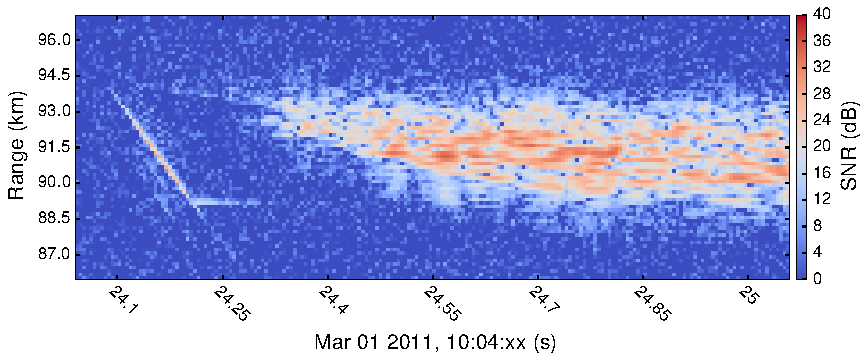
\includegraphics[trim=0px 20px 0px 3px,clip]{head_and_flare_mf_rti_0}
  \caption{Barker-13 pulse (13$\mu$s)}
  \label{fig:meteor_barker13_mf}
 \end{subfigure}
 
 \vspace{0.5\baselineskip}
 \begin{subfigure}{\textwidth}
  \centering
  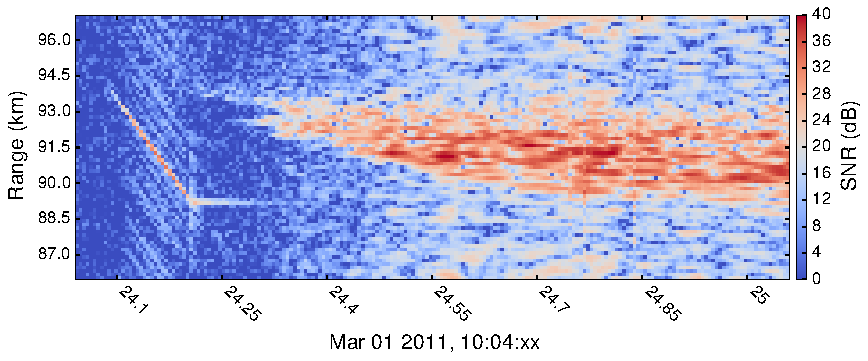
\includegraphics[trim=0px 20px 0px 3px,clip]{head_and_flare_mf_rti_1}
  \caption{Minimum peak sidelobe pulse (51$\mu$s with 51 bauds)}
  \label{fig:meteor_msl_mf}
 \end{subfigure}
 
 \vspace{0.5\baselineskip}
 \begin{subfigure}{\textwidth}
  \centering
  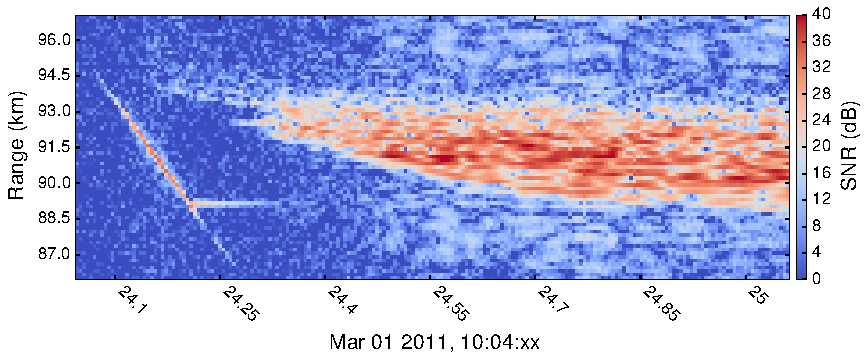
\includegraphics[trim=0px 20px 0px 3px,clip]{head_and_flare_mf_rti_3}
  \caption{LFM chirp (51$\mu$s with 1 MHz frequency sweep)}
  \label{fig:meteor_lfm_mf}
 \end{subfigure}
 \caption[Meteor head and trail measured with coded pulses]{\emph{Meteor head and trail measured with coded pulses.} These figures show the peak-frequency-response matched filter results for different waveforms over one second of 1$\mu$s-sampled data taken with the 50 MHz Jicamarca radar. Range sidelobes from the codes create significant ambiguity and make interpretation difficult.}
 \label{fig:meteor_msl_lfm}
\end{figure}%
Since these are RTI plots, the matched filter results show the peak-frequency-response filter for each pulse. Because of that, the artifacts that crowd the plot are mostly the zero-frequency-axis range sidelobes for each code. Unsurprisingly, the uncoded pulse's sidelobes completely dominate the output when that code is used. The meteor trail in particular appears as a high SNR mess. The Barker-13 code produces much more manageable sidelobes where the head echo and primary regions of trail scatter are clearly visible. Unfortunately, the Barker-13 pulse is necessarily much shorter in length, and the reduced sensitivity is evident with lower overall SNR. The minimum sidelobe code has higher SNR while keeping the acceptable sidelobe performance of the Barker-13 code. However, the sidelobes are still clearly significant and can easily obscure weaker scatterers, especially when the scatterers are shifted in frequency and have to contend with the very significant off-axis sidelobes. Finally, the LFM chirp produces the cleanest-looking results, an outcome which is not surprising given its ambiguity function. It is important to note though that they come at the cost of range bias and loss of frequency information; those shortcomings are only mitigated in this instance by the use of the other codes to determine the proper decoding frequency.

The example meteor head echo and trail are particularly well-behaved because they occur separately and without any other targets interfering. Even though that is usually the case when only meteors are observed, sidelobes are the primary reason that many outstanding ionospheric science questions cannot be satisfactorily answered with current techniques. Any time multiple or distributed scatterers are observed, sidelobes obscure or bias the measurements. The prior examples of challenging meteor phenomena, flaring in Figure \ref{fig:meteor_scattering_example} and fragmentation in Figure \ref{fig:mathews_fragmentation}, are just two important cases. Matched filtering is one way to decode coded radar measurements, and its limitations are clear. What is needed is a new decoding technique that keeps the benefits of the matched filter, sensitivity and efficient computation, but does not produce sidelobes. The problem in developing such a technique is that there are an infinite number of ways to construct a delay-frequency target scene that matches the measurements, and we're looking for the one that is both correct and sidelobe-free.

\section{Current Techniques}
\label{current_radar_techniques}
\subsection{Sidelobe Mitigation}
Accounting for matched filter ambiguity is not a new problem, and there are many ways it has been addressed in the past. The most obvious method is the one we've already covered: sidelobe mitigation through the selection of well-behaved codes. Obviously waveforms like the Barker codes, minimum peak sidelobe codes, and LFM chirp have more manageable sidelobes than an uncoded pulse or even most other waveforms. This is by design, as those codes were formulated to have either the minimum peak range sidelobes or to be insensitive to frequency shifts. Their typical use in applications such as satellite tracking, where sensitivity is essential and point-like targets are the norm, demonstrates their effectiveness in particular circumstances. As we've seen, though, these codes are only effective when it is simple to ignore the sidelobes that do remain. It is especially hard to ignore those sidelobes when targets with multiple Doppler frequency shifts are present, since the off-zero-axis delay-frequency sidelobes are quite significant. This is a consequence of the codes being designed to minimize only the zero-frequency-axis range sidelobes. Codes employing a larger set of phases, such as quadriphase codes \autocite{DLOV08}, show promise in improving performance over the widespread binary-phase codes \autocite{VLR+13}, but they still have many of the same fundamental sidelobe limitations.

\subsection{Alternating Codes}
Alternating codes are an approach to completely removing sidelobes by using a complementary set of codes over multiple pulses \autocite{LH87,Sul93,MVM08}. When the multi-pulse data is summed together, sidelobes from the individual codes cancel out to make the set sidelobe-free. Since incoherent scatter radars must already integrate over multiple pulses to get significant signal, alternating codes are widely used to measure incoherent scatter from the background ionosphere. As that application alludes to, alternating codes are an effective approach when target properties remain stationary over the time it takes to transmit the code set. Unfortunately, that is a constraint that limits flexibility and rules out many cases of interest.

\subsection{Inverse Filters}
It is also possible to leave matched filters behind altogether and use an alternative filtering or inversion technique. An inverse filter is one designed specifically to produce no range sidelobes at a point target's particularly frequency shift. Theoretically, inverse filters are infinite in length, but practically, finite-length truncation can achieve nearly indistinguishable inversion behavior. Like the matched filter, the inverse filter is a function of the transmitted code and is performed by a simple linear filtering operation on the received radar data. Since they are not optimal-SNR matched filters, however, inverse filters result in a loss of sensitivity that depends on the particular code used. Recent work into so-called perfect codes \autocite{LDPO09} make inverse filters more attractive, since perfect codes are designed so that the inverse filter is also the matched filter. One reason that perfect codes are not more widespread is that they require amplitude modulation in addition to phase modulation for each baud, and this can be difficult to achieve in practice.

Another reason that perfect codes are not more widespread is that inverse filters still produce significant sidelobes when the target frequency does not match the decoding frequency. This is evident in Figure \ref{fig:inverse_ambiguity_comparison}, which compares the ambiguity function for the Barker-13 code for both the matched filter and the inverse filter.
\begin{figure}[tpb]
 \centering
 \begin{subfigure}{0.5\textwidth}
  \centering
  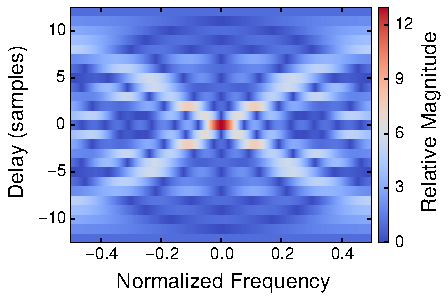
\includegraphics{ambiguity_barker13}
  \caption{Barker-13 matched filter ambiguity}
  \label{fig:barker13_matched_ambiguity}
 \end{subfigure}%
 \begin{subfigure}{0.5\textwidth}
  \centering
  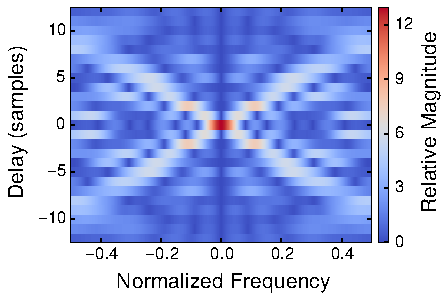
\includegraphics{ambiguity_inverse_barker13}
  \caption{Barker-13 inverse filter ambiguity}
  \label{fig:barker13_inverse_ambiguity}
 \end{subfigure}
 \caption[Comparison of matched and inverse filter ambiguity functions]{\emph{Comparison of matched and inverse filter ambiguity functions.} These delay-frequency images show the ambiguity function magnitude with $N=512$ frequencies for the Barker-13 code. The \textbf{(\subref{fig:barker13_matched_ambiguity})} matched filter and \textbf{(\subref{fig:barker13_inverse_ambiguity})} inverse filter ambiguities are nearly identical apart from the zero-frequency axis, indicating that the inverse filter is no more useful when decoding targets with unknown frequency shifts.}
 \label{fig:inverse_ambiguity_comparison}
\end{figure}%
On the global scale of the entire delay-frequency space, the two ambiguity functions look extremely similar. The Barker-13 code does not suffer much SNR loss due to the inverse filter, but most of the sidelobes remain as significant as with the matched filter. Only by examining the zero-frequency axis is it apparent that the inverse filter does indeed produce no range sidelobes when it matches the target's frequency. In the common case when the target Doppler shift is unknown or multiple frequencies must be decoded, the inverse filter provides no advantage.

\subsection{Inversion}
Framing decoding as a standard inversion problem is the most general approach to handling coded waveforms, and this is the tactic that we will use in the subsequent chapters. First, however, we must note the existing methods that perform this type of waveform inversion. The common link in these approaches is the formulation of a forward model that translates the true radar scene into measurements. Once this model is known, it can be inverted using an optimization routine to recover the ambiguity-free radar scene from the received signal. The amplitude domain inversion method of \textcite{VLV08} is similar to the one that we will develop later. The radar scene is decomposed over delay-frequency space just as with the matched filter, and a linear equation relates the delay-frequency scattering to the received signal. Just as we noted earlier, this model has an infinite number of solutions in the general case. However, \textcite{VLV08} take the approach of limiting the analysis to targets with a narrow delay/range. The problem is then well-posed, and statistical inversion is achieved by maximizing the likelihood of the posterior distribution. Limiting the target to a known narrow range extent is akin to manually specifying that most of the delay space is free from significant scatterers. It is a range sparsity assumption like the one that we will use, but their method requires the user to manually specify the target model whereas our approach is fully automated. That step in increased generality is significant for practical application.

Other existing inversion methods work with autocorrelation lag products of the received signal instead of the measurements directly. Lag profiles, the autocorrelation lags as a function of range, suffer from the same range ambiguity due to coding as the direct measurements. \textcite{DLN04} and \textcite{VLN+08} describe how to invert the lag profiles by solving a linear maximum a posteriori (MAP) matrix equation. Another MAP method is applied for lag profile inversion by \textcite{NKKS08}, with the difference being the use of regularization to stabilize the solution. These methods are hindered by the fact that they need either low SNR or the integration of many pulses in order to be applicable, otherwise the noise in the lag profile measurements is not Gaussian \autocite{LVV08}. In practice, this constraint has limited their use to the decoding of the inherently low-SNR incoherent scatter measurements.